\documentclass[journal]{IEEEtran}
\renewcommand\thesection{\arabic{section}} 
\renewcommand\thesubsectiondis{\thesection.\arabic{subsection}}
\renewcommand\thesubsubsectiondis{\thesubsectiondis.\arabic{subsubsection}}
\renewcommand\theparagraphdis{\arabic{paragraph}.}
\usepackage{xcolor,soul,framed} %,caption
\colorlet{shadecolor}{yellow}
\usepackage[pdftex]{graphicx}
\graphicspath{{../pdf/}{../jpeg/}}
\DeclareGraphicsExtensions{.pdf,.jpeg,.png}
\usepackage[cmex10]{amsmath}
\usepackage{array}
\usepackage{mdwmath}
\usepackage{mdwtab}
\usepackage{eqparbox}
\usepackage{url}
\usepackage{amsfonts}
\hyphenation{op-tical net-works semi-conduc-tor}
\usepackage{graphicx}
\usepackage{hyperref}
%
%=== TITLE & AUTHORS ====================================================================
%
\begin{document}
\bstctlcite{IEEEexample:BSTcontrol}
    \title{
\includegraphics[width=2.5in]{photo/0_cityu} \\
    Image Classification on the CIFAR10 Dataset\\
     \textit{Working Paper for CS4487 Machine Learning}
     }
  \author{BOHNSTEDT 	Timo ,
      L\"OHR Tim\\ 
}
\markboth{Project Report
Machine Learning CS4487 
}{Roberg \MakeLowercase{\textit{et al.}}}

% ====================================================================
\maketitle
% === ABSTRACT 
\begin{abstract}
%\boldmath
As part of our final group project, students shall implement a neural network to gain a better understanding of machine learning in practise. To achieve our goal, we try to get the best possible accuracy. To fully understand this dataset and the classification problem, we provided a detailed description about the task and its problems. For having a broader understanding of what research contributes to this task of image recognition, we introduce a summary of the latest publications and developments around the image classification field. For our implementation, we decided to use a VGG16 model architecture. We go into detail about our model architecture and explain all of its components and corresponding layers. In the end we analyse the results of our training process and compare it with similar implementation and the state-of-the-art models. 
\end{abstract}

% === KEYWORDS 
\begin{IEEEkeywords}
\hl{cifar10, machine learning, data science, image classification}
\end{IEEEkeywords}

\IEEEpeerreviewmaketitle

% === I. Problem description ============================
\section{Problem Description}
\label{sec:problemDescription}
\IEEEPARstart{I}{}n our course Machine Learning at the City University of Hong Kong, Dr Kede teached us the fundamental mathematical knowledge to solve machine learning tasks. Furthermore, we improved our ability to use this knowledge while working on Jupyter Notebook tutorials, which were provided by Dr Kede and his assistant PhD students. To proof our learning progress in the theoretical and practical field, we are working on a group project. To solve an image classification task, we use the widely used dataset  "CIFAR10" \cite{echersly}\cite{mostpopular}. The original dataset consists of 60000 coloured images of objects from 10 classes, with 6000 images per category. There are 50, 000 training images and 10, 000 test images. To compare our work with other groups, we are using the following evaluation criteria:
\begin{equation}
Acc(f,D) = \frac{1}{m}\sum_{m}^{i=1} \mathbb{I} \left [ y^{(i)} =f(x^{()i)})\right ]
\label{acc}
\end{equation}
\begin{figure}
  \begin{center}
  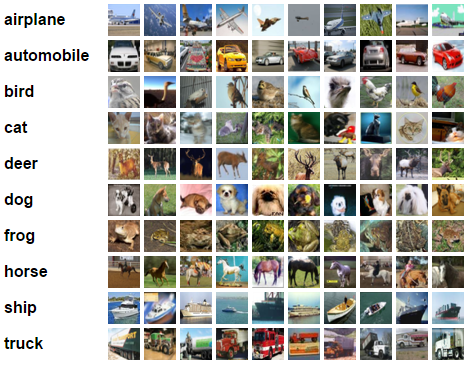
\includegraphics[width=3.5in]{photo/image32.png}\\
  \caption{CIFAR10 dataset}\label{cifar10}
  \end{center}
\end{figure}
\noindent When working on machine learning tasks with the Python programming language, the three most commonly used frameworks are Keras, PyTorch and Tensorflow \cite{favFrameworks}. Keras itself is based on tensorflow and hence it is easier to use, but does not provide to full capacity of the entire tensorflow framework\cite{DlKeras}. Recently Tensorflow 2.0 got released, so we decided in favor of that and chose Keras, because it impacts the performance of Keras itself too. 
% === II. Literature Survey ============================
\section{Literature Survey}
\noindent As mentioned in our \hyperref[sec:problemDescription]{"Problem Desciption"}, for an image recognition task the CIFAR10 dataset is quite popular. The archive of the Cornell Univerity provides a huge amount of papers regarding the latest machine learning research. We found 336 publications as we searched for the term "CIFAR10" . There are two independent and well known websites \footnote{\href{https://paperswithcode.com/sota/image-classification-on-cifar-10}{https://paperswithcode.com/sota/image-classification-on-cifar-10}} \footnote{\href{https://benchmarks.ai/cifar-10}{https://benchmarks.ai/cifar-10}} which rank annually the most recent performances for the image classifcation task on CIFAR10. The rankings are mostly referring to the overall test accuracy or the total loss \cite{echersly}. For simplification, we are relating to the classification of the web page "paperswithcode.com" \footnote{\href{http://arxiv.org/}{http://arxiv.org/}}. In the following we shortly introduce some of the most successful architectures which are at the top of the leaderboard. \\

\begin{figure}
  \begin{center}
  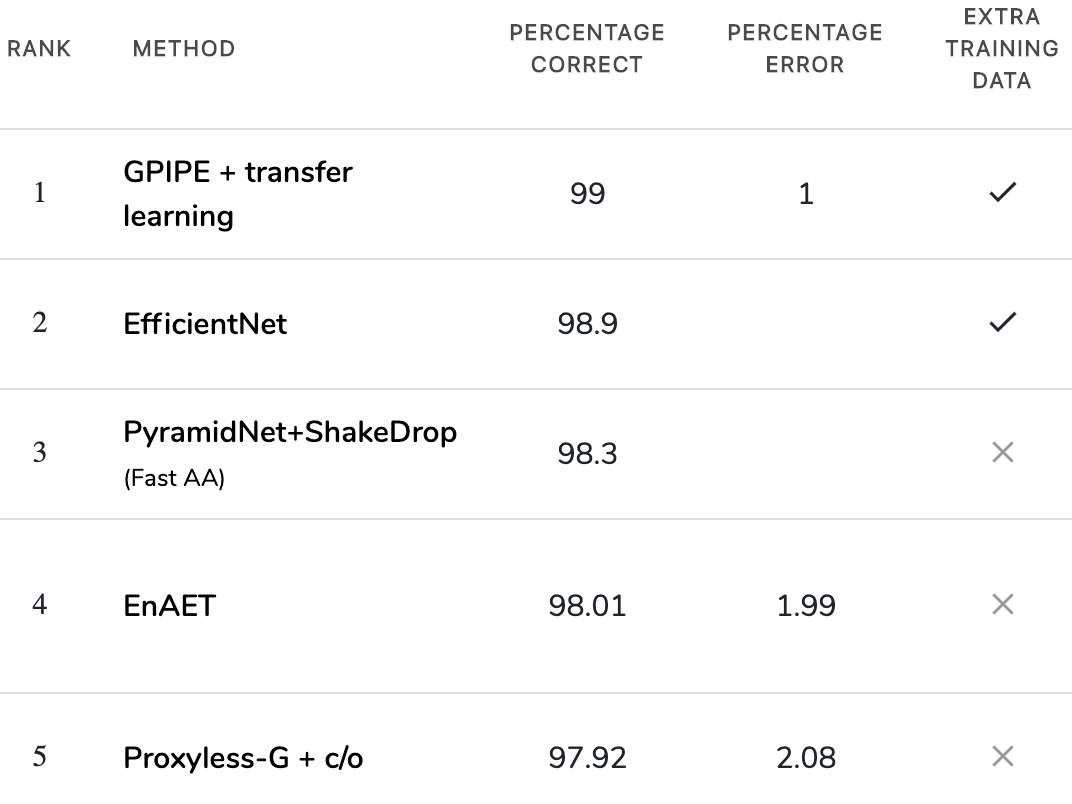
\includegraphics[width=3.5in]{photo/related_work.png}\\
  \caption{CIFAR10 Leaderboard Top 5, 2019.12.13}\label{leaderboard}
  \end{center}
\end{figure}

\subsection{GPipe}
In smaller experiments the training process for a model is relatively fast, whereas the training process for a model with an upscaled complexity consumes dramatically more time.
\cite{Yao2017ComplexityVP}.\\
Researchers at Google implemented a machine learning library which offers parallelization for the training process of a machine learning model. The GPipe uses mini-batch gradient descent and pipeline parallelism. The goal is that \(k\) accelerators can calculate a defined part of the model \(k\). If we can split our model into \(k\)  parts, we are able to scale the training process even higher \cite{GPipe}. This leads to an outstanding performance boost in machine learning tasks, such as image recognition\cite{perfGPipe}. The researchers could verify their work by using real word datasets like the CIFAR10. They reached an accuracy of 99\% \cite{GPipe} with this dataset. 
\subsection{EfficientNet}
While we could use the GPipe for running our complicated and colossal model parallel, EfficientNet trys to get the same result in a more efficient way\cite{EfficientNet} . So, instead of using more resources, they introduce the idea of a super-efficient method to reach better or similar results for using fewer resources with already existing neural network architectures\cite{EfficientNet}. For example, they increased the accuracy of the ResNet up to 10\% with almost not using any extra resources.
\subsection{PyramidNet}
In many modern CNN architectures, the feature map dimensions are not increased until they are confronted with a downsampling layer.
The key idea of the PyramidNet was introduced in the working paper \textit{Deep Pyramidal Residual Networks} \cite{lim2019fast}. This architecture concentrats on the feature
map dimensions, in particular it increases the dimensions gradually instead of increasing them sharply at each residual unit with a downsampling task. Additionally, this network architecture is a mixture of both plain and residual networks \cite{lim2019fast}. The team also introduced a \textit{novel residual unit} which can improve the performance of an ResNet architecture even more dramatically. 
In conclusion is the PyramidNet outperforming the normal ResNet and the DenseNet \cite{lim2019fast}.
%
% === III. Technical Details ============================
%
\section{Technical Details}
\label{sec:techDetails}
\subsection{Preprocessing}
\subsubsection{Data Augmentation}
\noindent Data augmentation describes the method of creating new data points by transforming the original data. If we look at images, this can be proceeded for example by resizing, rotating, shifting, flipping and more.
With this process we can artificially increase the amount of data, eventhough we have limited access to only 50000 training data. 
This leads to an improved performance for our VGG model. \\
We use the \textit{ImageDataGenerator class} built-in function from Keras itself to perform this transformations. \\

\subsubsection{Normalization}
\noindent The goal of normalization is to scale every datapoint in such a way, that outliners cannot harm the rest of the datapoints. There are many possible ways to scale data e.g. MinMax-Scaling or Z-Score and all of them follow certain purposes. 
The MinMax-Scaling suffers from the so called \textit{outlier issue}.
We decided to choose the Z-Scoring, because the Z-score normalization is a strategy of normalizing data that avoids this outlier issue \cite{RN6}. \\
\begin{figure}
  \begin{center}
  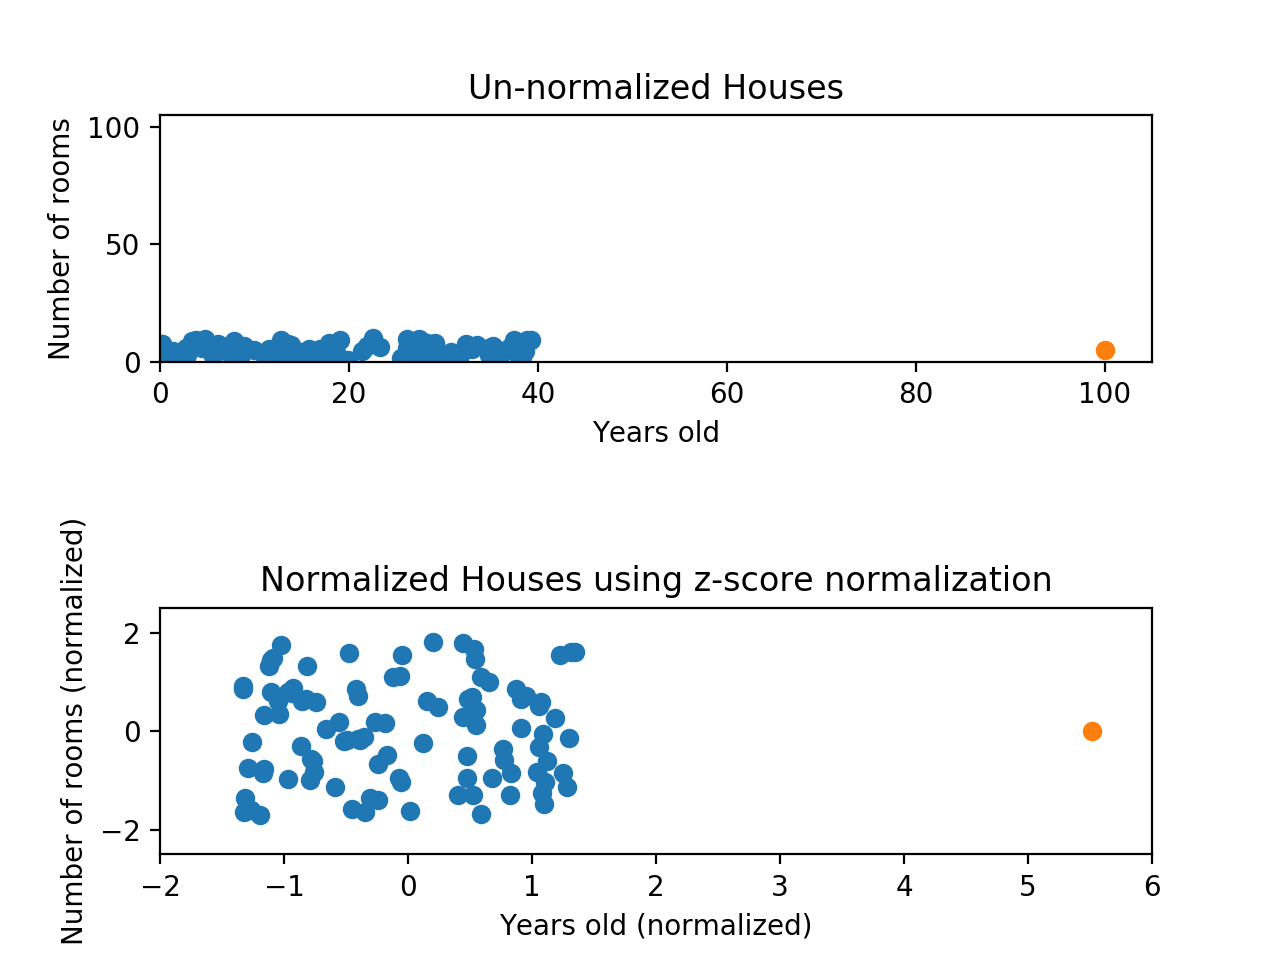
\includegraphics[width=3.5in]{photo/z-score.png}\\
  \caption{Z-Scoring}\label{zscore}
  \end{center}
\end{figure}
The Z-scoring \(\frac{value - \mu}{\sigma}\) transforms example data as shown in the figure \ref{zscore} \footnote{\href{https://www.codecademy.com/articles/normalization}{https://www.codecademy.com/articles/normalization}}.


\subsubsection{Categorical Output}
\noindent As the name of CIFAR10 already implies, does this dataset contain of ten different classes. There are ten different animals given by the creators of this dataset. To predict one of those animals with the trained model, the model outputs ten different values, each represents the probability of being one of the animals respectively. 
We convert the aranged numbers from one to ten 50000, 1) into a binary output class matrix (50000, 10). Each row in this matrix values one for the desired animal. E.g. animal number three will be transformed into [0 0 1 0 0 0 0 0 0 0].
If we didn't convert our labels into this format, we could not resolve back the probability for each animal and would lose information to improve. \\

\subsection{Model}
\noindent To solve the image classification task, we are using a convolutional neuronal network (CNN). CNN's are a particular case of feed-forward neural networks \cite{Goodfellow-et-al-2016}. On a very fundamental level, we can say that a feed-forward neural network - as the most machine learning models - is a function. The function of a feed-forward neural network can simply be descriped as \(y = f(x, \o )\) . CNN's and feed-forward neural networks are estimating parameter values. So for \(y = f(x, \o )\) we estimate the parameter \(\o \) \cite{Goodfellow-et-al-2016}. Through those estimated parameter values we are receiving a function back with the smallest possible difference between the predicted output values and the defined output values. A function that measures the difference between the expected - and the defined output is a so - called loss function \cite{Goodfellow-et-al-2016}. The problem description gives already a mathematical definition \eqref{acc} from the accuracy loss function which is used by us. 
CNN's and classical feed-forward neuronal networks differ in their basis of calculation. Feed-forward neural networks are using matrix multiplication, whereas CNN's are using convolutions. Convolutional layers, pooling layers, and fully-connected layers are specific layers for a CNN \cite{LeCun1998}. \\
\subsubsection{Model Architecture}
We decided to use the VGG16 model architecture. In 2014, an implementation of the architecture won the ILSVR(Imagenet) competition. As we could already see in figure \ref{leaderboard} that there are quite impressive results, we still decided to use this classic example. The complexity is rather small in comparison to other designs which are provided in the ranking. Note that - as  mentioned in the \hyperref[sec:problemDescription]{"Problem Desciption"}, the goal of our project was not to get an outstanding result of the accuracy. The main goal was  to understand the principals behind deep learning and to get a feeling of what the state of the art (in image recognition) is. So, because the VGG16 is known as the best visualizable model architecture, we thought it would be the best choice to accomplish our goal in this way. The model architecture is also known for getting rid of a vast amount of hyper-parameters. Instead, it is focusing on tiny filter size and a small strate. The technical details \hyperref[sec:techDetails]{"Problem Desciption"}, of the different layers are providing more details about its implementaiton. 
\subsubsection{Convolutional Layers}
\noindent The convolutional Layer performs the extracting of features from the input matrix into a feature map. For this procedure, we use matrix multiplication in form of the dot product and a filter (feature detector, kernel) \cite{Goodfellow-et-al-2016}. 

\begin{figure}
  \begin{center}
  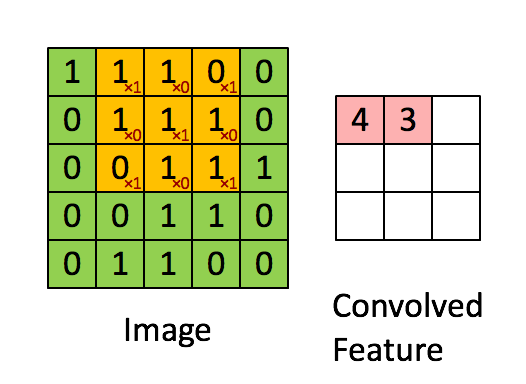
\includegraphics[width=3in]{photo/cnn.png}\\
  \caption{Feature Map derived from http://deeplearning.stanford.edu}\label{featuremap}
  \end{center}
\end{figure}

In picture \ref{featuremap} you can see a calculation example of how convolution is applied to a matrix. We are iterating with the filter over the matrix, calculating the scalar product and writing the result into a feature map. An activation function like the rectified linear unit (ReLU) normalizes the feature map after we performed the convolution. Normalization guarantees a feature map which is not a linear transformation of its input value. If this is the case, we only have a linear problem which can be easily solved, but with a wrong result. In other words, the input values get just multiplied by coefficients. Note that there are plenty of reasons for activation functions in a neuronal network. We are giving a closer look at this topic at our section \hyperref[sec:activationFunctions]{"Activation Functions"}. In Figure \ref{featuremap1} you can see how our pictures had changed after applying the first convolutional layer, before and after doing normalization.  \\

\begin{figure}
  \begin{center}
  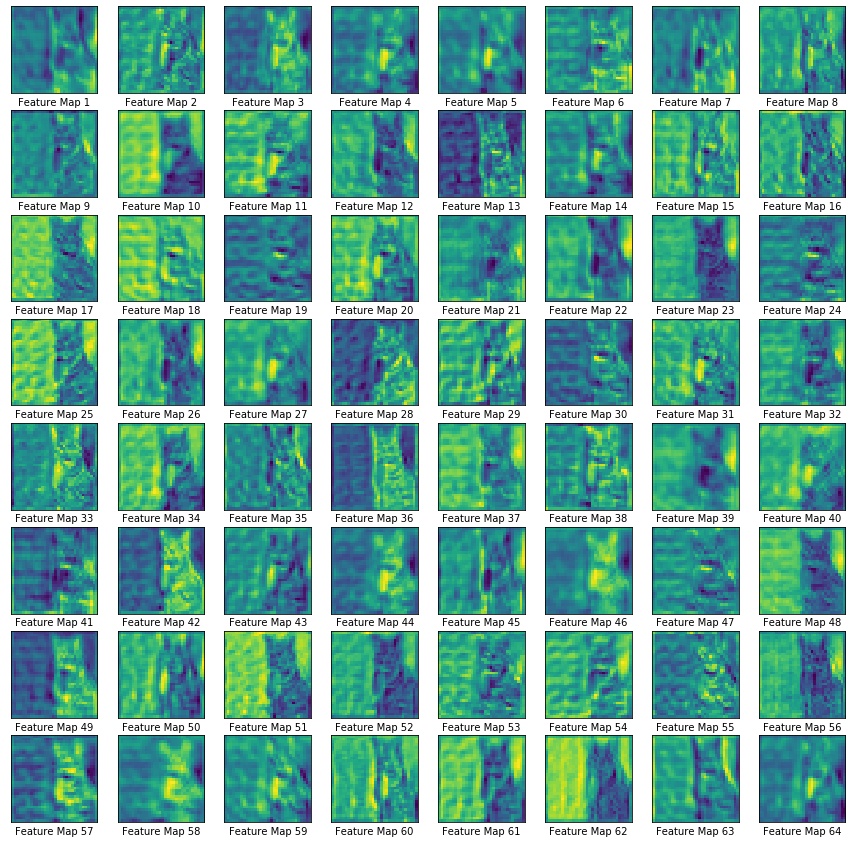
\includegraphics[width=3in]{photo/feature_map1.png}\\
  \caption{Feature Map from CNN Layer 1}\label{featuremap1}
  \end{center}
\end{figure}

\begin{figure}
  \begin{center}
  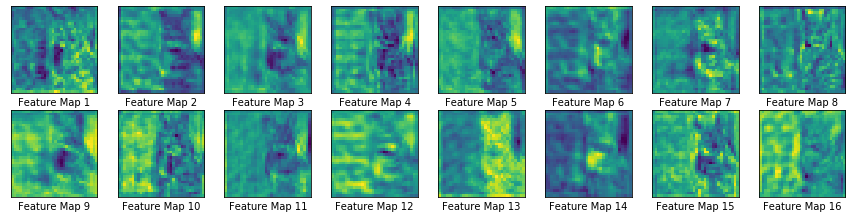
\includegraphics[width=3in]{photo/feature_map2.png}\\
  \caption{Feature Map from CNN Layer 2}\label{featuremap2}
  \end{center}
\end{figure}

This represents the 64 first feature maps of a random picture from the dataset. We can observe that the filters already focus on certain points on the cat's body. We further used this feature map as input for the second CNN layer. The output of the second feature map (figure \ref{featuremap2}) further sharpens the filters. For example we can see that feature map 2 until 5 focus on the cat itself, whereas map 8 puts it focus on the cats ears. \\

\subsubsection{Pooling Layers}
\noindent It is common to periodically add a pooling layer in-between the convolutional layers. Its function is to avoid overfitting and step by step reduce the size of the input image by reducing the amount of parameters and computations of the network. We use three pooling layers with filters of size 3x3 applied with a stride of 0 and a padding set to \textit{same}. This downsamples every depth slice in the input by 2 along both width and height, discarding 50\% of the activations. \\
\subsubsection{Fully-Connected Layers}
\noindent The Dense layer is the last layer of our model. It is also called the \textit{fully connected layer}. Neurons in the fully connected layer have full connections to all activations in the previous layer, as in the normal neural networks. Their activation functions will then be computed by a matrix multiplication which is followed by a bias offset. 
For the ten different animals we repectively have ten fully connected neurons in the dense layer. \\
\subsubsection{Kernel Regularization}
\noindent There are many different regularizations to prevent the neural network from overfitting. For our project we chose the \textit{L2 regularization}, because it is the most common form.
It can be integrated by penalizing the squared magnitude of all parameters directly in the objective. So, for every weight \textit{w} in the network, the term \(\frac{1}{2} \lambda w^2\) gets added to the objective, where \(\lambda \) is the regularization strength. It's usual to see \(\frac{1}{2}\) in the front, because then the gradient of this term with respect to \textit{w} is simply \(\lambda w\) instead of \(2 \lambda w\). The L2 penalizes the peaky weight vectors and prefers the diffuse weight vectors \cite{RN4}. During the gradien descent weight update, the L2 regularization means, that every weight is decayed linearly (\textit{w += -lambda * w}) towards zero. \\
\subsubsection{Batch Normalization}
\noindent A recently developed technique by Ioffe and Szegedy \cite{RN4} called Batch Normalization  properly initializes neural networks by explicitly forcing the activations throughout a network to take on a unit gaussian distribution at the beginning of the training. Normalization is a simple differentiable operation. 
It allowes to use higher learning rates at the beginning and is less vulnerable to a bad initialization. In other words, neural networks that implement batch normalization layers are significantly more robust. Additionally, batch normalization can be interpreted as a preprocessing step on every layer of the network. Batch normalization yields in general a substantial improvement in the training process. \\
\subsubsection{Activation Functions}
\label{sec:activationFunctions}
\noindent There a couple of widely used activation functions like tanh, sigmoid function, ReLU or the ELU. For our model we decided to use the \textit{ReLU} activation function. The Rectified Linear Unit (ReLU) has become very popular in the last few years. It computes the function \(f(x)=max(0,x)\). In other words, the activation is simply thresholded at zero. There are plenty of pro's and con's for the ReLU:
\begin{itemize}
\item (+) Compared to tanh/sigmoid neurons that need to compute expensive operations  like the exponentials, the ReLU can be implemented by directly thresholding a matrix of activations at zero.
\item (+) It was found to notably accelerate the convergence of stochastic gradient descent (SGD) compared to the tanh/sigmoid functions. That is, because of its linear, non-saturating form.
\item (-) Sadly, ReLU units can be weak during training and possibly “die”. For example, a large gradient streaming through a ReLU neuron could cause the weights to update in a dead end, so that it will never activate again. If this happens, then the gradient streaming through the unit will forever be zero. The ReLU units can irreversibly die during training since they can get eliminated off the data manifold. With a good scheduling setting of the learning rate this is less likely to happen. \\
\end{itemize}
\subsubsection{Loss function}
\noindent Our compiled Keras model uses the \textit{cross-entropy-loss}. 
\begin{equation}
L_{i} = f_{y_{i}} + log \sum_{j} e^{f_{j}}
\end{equation}
where we are using the notation \(f_{j}\) to mean the \textit{j-th} element of the vector of class scores \textit{f}. The full loss for the dataset is the mean of \(f_{i}\) over all training examples together with a regularization term \textit{R(W)}.
The cross-entropy loss, or also called log loss, measures the performance of our classification model with the output as probability values between zero and one. The cross-entropy loss increases as the predicted probability diverges from real value labels.
\subsubsection{Optimizer}
\noindent There are many possible optimizer suitable for our task. The common ones are the RMSprob, Adam or the stochastic gradient descent (SGD). We decided to use the SGD
to minimize the loss by computing the gradient with respect to a randomly selected batch from the training set. This method is more efficient than computing the gradient with respect to the whole training set before each update is performed.
\begin{equation}
\frac{\partial p_i}{\partial a_j}=\left\{\begin{matrix} p_i(1-p_i) & if & i=j\\ -p_j p_i & if & i\neq j \end{matrix}\right.
\end{equation} \\
\begin{equation}
\frac{\partial L}{\partial o_i}=p_i-y\_oh_i
\end{equation} 
For the derivation of the cross entropy loss, \textit{y\_oh} is the one-hot encoded representation of the class labels.
\subsubsection{Softmax}
\noindent The softmax normalizes the class probabilities to one and it has a probabilistic interpretation. 
\begin{equation}
f_{j}(z) = \frac{e^{z_{i}}}{\sum_{k} e^{z_{k}}}
\end{equation}
The exponential values can very quickly explode to an infinite large number, for example \(e_{1000}\). To fix this issue, it takes a one-dimensional vector of arbitrary length (in \textit{z}) and puts it into a vector of values between zero and one that sum together to one. The cross-entropy loss that includes the softmax function, hence to minimize the cross-entropy-loss between the estimated class probabilites. \\
\subsubsection{Flatten}
In between the convolutional layer (CNN) and the fully connected layer (Dense), there is a \textit{Flatten layer}. The Flattening layer transforms a two-dimensional matrix of features into a one-dimensional vector that can be respectively streamed into the fully connected neural network classifier, which are our ten fully connected animal neurons. \\
%
% === IV. Result Analysis============================
%
\section{Result Analysis}
\subsection{Settings}
As mentioned in the model architecture, our implementation of the VGG16 network is still state of the art, but no longer among the very best of its field. Even more, we want to point out its difficulties and significant problems. As we look at our training process, we could see two things. First, the estimated time of our epochs is around 30 Minutes if we train it on our MacBook without Nvidia graphicscard. So, if we want to train 125 epochs to gain the best possible result without overfitting our model, we would need 62,5 hours. This is obviously too long. \\ One possible way is to translate the \textit{.ipynb} format into \textit{.py} format, because we can then run the model as a background job on a tiny server. The tiny server has a similar training time, but can be trained in the background. 
The best solution for us was to use a server from the Amazon Web Services (AWS). We rented the \textit{Deep Learning AMI (Amazon Linux 2) Version 26.0} \footnote{\href{https://eu-west-1.console.aws.amazon.com/}{https://eu-west-1.console.aws.amazon.com/}}. On this server we can run the Jupyter Notebook in the background and use the portforward function from the SSH connection to show the user interface (UI) of the jupyter notebook on our Macbooks. In this way we can train the model as learned from the CS4487 lecture. \\
The AMI Server from Amazon gets shipped with multiple python environments which can be activated manually. We chose the \textit{p36 Tensorflow Kernel} to activate the neccessary packages.
Under this setting our model needs approximately only 3~4 hours to be trained. \\ 
\subsection{Model Analysis}
Besides the difficulties we had, if we would consider improving our accuracy with the VGGNet, we could say that our model does a good job due to overfitting as you can see in Figure XYZ. This achievement is mostly because of our attempted to avoid overfitting while using a weight decay, kernel regularizer and batch normalization. The figure XYZ furthermore shows, that no matter how many more epochs we train, the accuracy will not further increase.

% ============================================
\ifCLASSOPTIONcaptionsoff
  \newpage
\fi
\bibliographystyle{IEEEtran}
\bibliography{IEEEabrv,Bibliography}
\vfill
\end{document}